\section[Resultados]{Resultados}

\begin{frame}[t,allowframebreaks]
\frametitle{Resultados}

    Para analisar os resultados, foram realizados tr�s conjuntos de
    testes:

    \begin{enumerate}
        \item links acessados ap�s 1 hora do rein�cio dos registros;
        \item links acessados ap�s 10 horas do rein�cio dos registros;
        \item links acessados ap�s 24 horas do rein�cio dos registros.
    \end{enumerate}

    Para precis�o dos resultados, a equa��o de subtra��o de ferom�nio foi ajustada para
    relevar at� 5 casas decimais.

    \begin{table}
    \centering \caption{Diferen�a de tempo inicial entre as p�ginas}
    \label{tab:diftempo}
    \begin{scriptsize}
    \begin{tabular}{|l|l|l|l|}
    \hline
    pg & �ltimo-acesso & dif & qf0 \\
    \hline
    1 & 12:31 & 0min & 10 \\
    \hline
    2 & 12:31 & 0min & 20 \\
    \hline
    3 & 12:32 & 1min & 10 \\
    \hline
    4 & 12:33 & 2min & 10 \\
    \hline
    5 & 12:35 & 4min & 10 \\
    \hline
    6 & 12:35 & 4min & 20 \\
    \hline
    7 & 12:36 & 5min & 10 \\
    \hline
    8 & 12:36 & 5min & 10 \\
    \hline
    9 & 12:37 & 6min & 10 \\
    \hline
    10 & 12:38 & 7min & 20 \\
    \hline
    11 & 12:39 & 8min & 10 \\
    \hline
    12 & 12:39 & 8min & 10 \\
    \hline
    \end{tabular}
    \end{scriptsize}
    \end{table}

    \newpage

    Os par�metros iniciais do sistema tinham os valores:

    \begin{itemize}
        \item Tr�s grupos de interesse, sendo: 1=�ltimas not�cias; 2=Mundo; 3=Brasil;
        \item Constante que define a relev�ncia de um acesso $\xi$: 10;
        \item Taxa de evapora��o $\varphi$: 35.
    \end{itemize}

\end{frame}

\begin{frame}[t,allowframebreaks]
\frametitle{Links acessados ap�s 1 hora do rein�cio dos registros}

        \begin{table}[H]
        \caption{Links acessados ap�s 1 hora do rein�cio dos registros}
        \label{tab:resultadotr1h}
        \tiny{
            \begin{center}
                \begin{tabular}{|c|c|r|r|r|r|r|r|}
                \hline
                \# & origem-destino-grupo & qf it1 & qf it2 & qf it3 & qf it4 & qf it5 \\
                \hline
                \textcolor[rgb]{0.31,0.51,0.74}{\textbf{1}} & \textcolor[rgb]{0.31,0.51,0.74}{\textbf{1-1-1}} & \textcolor[rgb]{0.31,0.51,0.74}{\textbf{9,92858}} & \textcolor[rgb]{0.31,0.51,0.74}{\textbf{9,85717}} & \textcolor[rgb]{0.31,0.51,0.74}{\textbf{9,78568}} & \textcolor[rgb]{0.31,0.51,0.74}{\textbf{9,71423}} & \textcolor[rgb]{0.31,0.51,0.74}{\textbf{9,64282}} \\
                \hline
                \textcolor[rgb]{0.75,0.31,0.30}{\textbf{2}} & \textcolor[rgb]{0.75,0.31,0.30}{\textbf{1-2-1}} & \textcolor[rgb]{0.75,0.31,0.30}{\textbf{19,85715}} & \textcolor[rgb]{0.75,0.31,0.30}{\textbf{19,71432}} & \textcolor[rgb]{0.75,0.31,0.30}{\textbf{19,57134}} & \textcolor[rgb]{0.75,0.31,0.30}{\textbf{19,42845}} & \textcolor[rgb]{0.75,0.31,0.30}{\textbf{19,28563}} \\
                \hline
                3 & 1-3-1 & 9,92974 & 9,85947 & 9,78911 & 9,71877 & 9,64845 \\
                \hline
                4 & 1-4-1 & 9,9309 & 9,86177 & 9,79253 & 9,72331 & 9,65409 \\
                \hline
                5 & 1-5-2 & 9,93322 & 9,86638 & 9,7994 & 9,7324 & 9,66537 \\
                \hline
                6 & 5-6-2 & 19,86644 & 19,73277 & 19,59881 & 19,46482 & 19,33076 \\
                \hline
                7 & 5-7-2 & 9,93438 & 9,86869 & 9,80284 & 9,73696 & 9,67103 \\
                \hline
                8 & 5-8-2 & 9,93438 & 9,86869 & 9,80284 & 9,73696 & 9,67103 \\
                \hline
                9 & 1-9-3 & 20 & 19,99899 & 19,99677 & 19,99358 & 19,98937 \\
                \hline
                \textcolor[rgb]{0.61,0.73,0.35}{\textbf{10}} & \textcolor[rgb]{0.61,0.73,0.35}{\textbf{9-10-3}} & \textcolor[rgb]{0.61,0.73,0.35}{\textbf{19,8734}} & \textcolor[rgb]{0.61,0.73,0.35}{\textbf{19,7466}} & \textcolor[rgb]{0.61,0.73,0.35}{\textbf{19,61943}} & \textcolor[rgb]{0.61,0.73,0.35}{\textbf{19,49213}} & \textcolor[rgb]{0.61,0.73,0.35}{\textbf{19,36467}} \\
                \hline
                11 & 9-11-3 & 9,93786 & 9,87561 & 9,81316 & 9,75063 & 9,688 \\
                \hline
                12 & 9-12-3 & 9,93786 & 9,87561 & 9,81316 & 9,75063 & 9,688 \\
                \hline
                13 & 9-13-3 & 0 & 10 & 9,9994 & 9,99831 & 9,99671 \\
                \hline
                14 & 9-14-3 & 0 & 0 & 10 & 9,99951 & 9,99852 \\
                \hline
                \textcolor[rgb]{0.49,0.38,0.63}{\textbf{15}} & \textcolor[rgb]{0.49,0.38,0.63}{\textbf{9-15-3}} & \textcolor[rgb]{0.49,0.38,0.63}{\textbf{0}} & \textcolor[rgb]{0.49,0.38,0.63}{\textbf{0}} & \textcolor[rgb]{0.49,0.38,0.63}{\textbf{0}} & \textcolor[rgb]{0.49,0.38,0.63}{\textbf{10}} & \textcolor[rgb]{0.49,0.38,0.63}{\textbf{9,99949}} \\
                \hline
                16 & 9-16-3 & 0 & 0 & 0 & 0 & 10 \\
                \hline
                \end{tabular}
            \end{center}
        }
        \end{table}

        \begin{figure}[htb]
            \begin{center}
                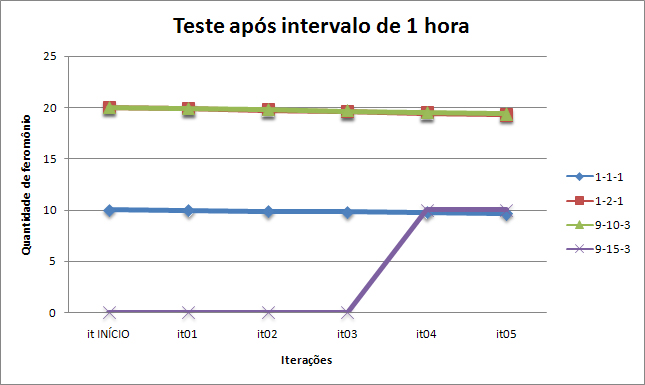
\includegraphics[width=10cm]{images/resultados/qtd_feromonio.jpg}
                \label{fig:qtd_feromonio}
                \caption{Gr�fico dos testes ap�s intervalo de 1 hora}
            \end{center}
        \end{figure}

\end{frame}

\begin{frame}[t,allowframebreaks]
\frametitle{Links acessados ap�s 10 horas do rein�cio dos registros}

        \begin{table}[H]
        \caption{Links acessados ap�s 10 horas do rein�cio dos registros}
        \label{tab:resultadotr10h}
        \tiny{
            \begin{center}
                \begin{tabular}{|c|c|r|r|r|r|r|r|}
                \hline
                \# & origem-destino-grupo & qf it1 & qf it2 & qf it3 & qf it4 & qf it5 \\
                \hline
                \textcolor[rgb]{0.31,0.51,0.74}{\textbf{1}} & \textcolor[rgb]{0.31,0.51,0.74}{\textbf{1-1-1}} & \textcolor[rgb]{0.31,0.51,0.74}{\textbf{9,31582}} & \textcolor[rgb]{0.31,0.51,0.74}{\textbf{8,67811}} & \textcolor[rgb]{0.31,0.51,0.74}{\textbf{8,08376}} & \textcolor[rgb]{0.31,0.51,0.74}{\textbf{7,5296}} & \textcolor[rgb]{0.31,0.51,0.74}{\textbf{7,01306}} \\
                \hline
                \textcolor[rgb]{0.75,0.31,0.30}{\textbf{2}} & \textcolor[rgb]{0.75,0.31,0.30}{\textbf{1-2-1}} &\textcolor[rgb]{0.75,0.31,0.30}{\textbf{18,63165}} & \textcolor[rgb]{0.75,0.31,0.30}{\textbf{17,35624}} & \textcolor[rgb]{0.75,0.31,0.30}{\textbf{16,16754}} & \textcolor[rgb]{0.75,0.31,0.30}{\textbf{15,05922}} & \textcolor[rgb]{0.75,0.31,0.30}{\textbf{14,02614}} \\
                \hline
                3 & 1-3-1 & 9,31691 & 8,68014 & 8,0866 & 7,53313 & 7,01717 \\
                \hline
                4 & 1-4-1 & 9,318 & 8,68217 & 8,08943 & 7,53664 & 7,02126 \\
                \hline
                5 & 1-5-2 & 9,32018 & 8,68624 & 8,09512 & 7,54371 & 7,02949 \\
                \hline
                6 & 5-6-2 & 18,64036 & 17,37247 & 16,19022 & 15,0874 & 14,05896 \\
                \hline
                7 & 5-7-2 & 9,32127 & 8,68827 & 8,09795 & 7,54723 & 7,03359 \\
                \hline
                8 & 5-8-2 & 9,32127 & 8,68827 & 8,09795 & 7,54723 & 7,03359 \\
                \hline
                9 & 1-9-3 & 20 & 19,99922 & 19,9977 & 19,99482 & 19,99089 \\
                \hline
                \textcolor[rgb]{0.61,0.73,0.35}{\textbf{10}} & \textcolor[rgb]{0.61,0.73,0.35}{\textbf{9-10-3}} & \textcolor[rgb]{0.61,0.73,0.35}{\textbf{18,64689}} & \textcolor[rgb]{0.61,0.73,0.35}{\textbf{17,38465}} & \textcolor[rgb]{0.61,0.73,0.35}{\textbf{16,20726}} & \textcolor[rgb]{0.61,0.73,0.35}{\textbf{15,10858}} & \textcolor[rgb]{0.61,0.73,0.35}{\textbf{14,08363}} \\
                \hline
                11 & 9-11-3 & 9,32454 & 8,69436 & 8,10647 & 7,55782 & 7,04593 \\
                \hline
                12 & 9-12-3 & 9,32454 & 8,69436 & 8,10647 & 7,55782 & 7,04593 \\
                \hline
                13 & 9-13-3 & 0 & 10 & 9,99963 & 9,99858 & 9,997 \\
                \hline
                14 & 9-14-3 & 0 & 0 & 10 & 9,99932 & 9,99811 \\
                \hline
                 \textcolor[rgb]{0.49,0.38,0.63}{\textbf{15}} &  \textcolor[rgb]{0.49,0.38,0.63}{\textbf{9-15-3}} &  \textcolor[rgb]{0.49,0.38,0.63}{\textbf{0}} &  \textcolor[rgb]{0.49,0.38,0.63}{\textbf{0}} &  \textcolor[rgb]{0.49,0.38,0.63}{\textbf{0}} &  \textcolor[rgb]{0.49,0.38,0.63}{\textbf{10}} &  \textcolor[rgb]{0.49,0.38,0.63}{\textbf{9,99947}} \\
                \hline
                16 & 9-16-3 & 0 & 0 & 0 & 0 & 10 \\
                \hline
                \end{tabular}
            \end{center}
        }
        \end{table}

        \begin{figure}[htb]
            \begin{center}
                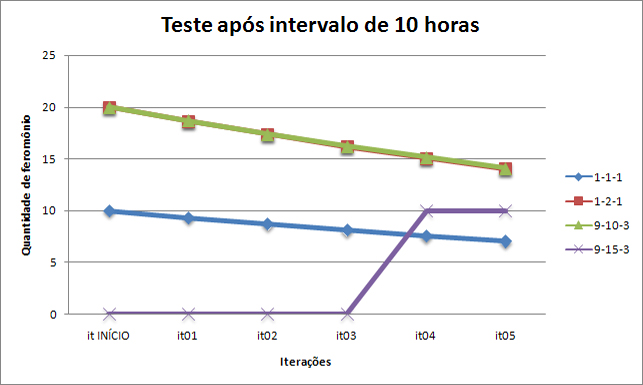
\includegraphics[width=10cm]{images/resultados/graf_teste10h.jpg}
                \label{fig:qtd_feromonio10h}
                \caption{Gr�fico dos testes ap�s intervalo de 10 horas}
            \end{center}
        \end{figure}
\end{frame}

\begin{frame}[t,allowframebreaks]
\frametitle{Links acessados ap�s 24 horas do rein�cio dos registros}

        \begin{table}[H]
        \caption{Links acessados ap�s 24 horas do rein�cio dos registros}
        \label{tab:resultadotr24h}
        \tiny{
            \begin{center}
                \begin{tabular}{|c|c|r|r|r|r|r|r|}
                \hline
                \# & origem-destino-grupo & qf it1 & qf it2 & qf it3 & qf it4 & qf it5 \\
                \hline
                \textcolor[rgb]{0.31,0.51,0.74}{\textbf{1}} & \textcolor[rgb]{0.31,0.51,0.74}{\textbf{1-1-1}} & \textcolor[rgb]{0.31,0.51,0.74}{\textbf{8,39057}} & \textcolor[rgb]{0.31,0.51,0.74}{\textbf{7,03988}} & \textcolor[rgb]{0.31,0.51,0.74}{\textbf{5,90639}} & \textcolor[rgb]{0.31,0.51,0.74}{\textbf{4,95517}} & \textcolor[rgb]{0.31,0.51,0.74}{\textbf{4,15693}} \\
                \hline
                \textcolor[rgb]{0.75,0.31,0.30}{\textbf{2}} & \textcolor[rgb]{0.75,0.31,0.30}{\textbf{1-2-1}} & \textcolor[rgb]{0.75,0.31,0.30}{\textbf{16,78114}} & \textcolor[rgb]{0.75,0.31,0.30}{\textbf{14,07976}} & \textcolor[rgb]{0.75,0.31,0.30}{\textbf{11,81278}} & \textcolor[rgb]{0.75,0.31,0.30}{\textbf{9,91034}} & \textcolor[rgb]{0.75,0.31,0.30}{\textbf{8,31387}} \\
                \hline
                3 & 1-3-1 & 8,39155 & 7,04153 & 5,90846 & 4,95749 & 4,15937 \\
                \hline
                4 & 1-4-1 & 8,39253 & 7,04317 & 5,91053 & 4,9598 & 4,16179 \\
                \hline
                5 & 1-5-2 & 8,3945 & 7,04647 & 5,91468 & 4,96445 & 4,16667 \\
                \hline
                6 & 5-6-2 & 16,78899 & 14,09293 & 11,82936 & 9,92889 & 8,33332 \\
                \hline
                4 & 5-7-2 & 8,39548 & 7,04812 & 5,91676 & 4,96677 & 4,1691 \\
                \hline
                7 & 5-8-2 & 8,39548 & 7,04812 & 5,91676 & 4,96677 & 4,1691 \\
                \hline
                8 & 1-9-3 & 20 & 19,99918 & 19,99758 & 19,99505 & 19,99151 \\
                \hline
                \textcolor[rgb]{0.61,0.73,0.35}{\textbf{10}} & \textcolor[rgb]{0.61,0.73,0.35}{\textbf{9-10-3}} & \textcolor[rgb]{0.61,0.73,0.35}{\textbf{16,79488}} & \textcolor[rgb]{0.61,0.73,0.35}{\textbf{14,10282}} & \textcolor[rgb]{0.61,0.73,0.35}{\textbf{11,84181}} & \textcolor[rgb]{0.61,0.73,0.35}{\textbf{9,94283}} & \textcolor[rgb]{0.61,0.73,0.35}{\textbf{8,34795}} \\
                \hline
                11 & 9-11-3 & 8,39842 & 7,05306 & 5,92298 & 4,97374 & 4,17642 \\
                \hline
                12 & 9-12-3 & 8,39842 & 7,05306 & 5,92298 & 4,97374 & 4,17642 \\
                \hline
                13 & 9-13-3 & 0 & 10 & 9,99961 & 9,99875 & 9,99739 \\
                \hline
                14 & 9-14-3 & 0 & 0 & 10 & 9,99953 & 9,99856 \\
                \hline
                 \textcolor[rgb]{0.49,0.38,0.63}{\textbf{15}} &  \textcolor[rgb]{0.49,0.38,0.63}{\textbf{9-15-3}} &  \textcolor[rgb]{0.49,0.38,0.63}{\textbf{0}} &  \textcolor[rgb]{0.49,0.38,0.63}{\textbf{0}} &  \textcolor[rgb]{0.49,0.38,0.63}{\textbf{0}} &  \textcolor[rgb]{0.49,0.38,0.63}{\textbf{10}} &  \textcolor[rgb]{0.49,0.38,0.63}{\textbf{9,99949}} \\
                \hline
                16 & 9-16-3 & 0 & 0 & 0 & 0 & 10 \\
                \hline
                \end{tabular}
            \end{center}
        }
        \end{table}

        \begin{figure}[htb]
            \begin{center}
                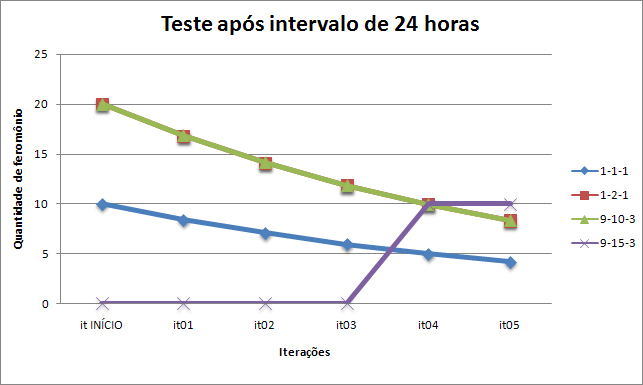
\includegraphics[width=10cm]{images/resultados/graf_teste24h.jpg}
                \label{fig:qtd_feromonio24h}
                \caption{Gr�fico dos testes ap�s intervalo de 24 horas}
            \end{center}
        \end{figure}
\end{frame}

\begin{frame}[t,allowframebreaks]
\frametitle{Diferen�a de ferom�nio nos testes efetuados}

        \begin{table}[H]
        \caption{Diferen�a de ferom�nio nos testes efetuados}
        \label{tab:testesdiferencas}
        \tiny{
            \begin{center}
            \begin{tabular}{|l|l|l|l|l|l|}
            \hline
            \multicolumn{1}{|c|}{Origem} & \multicolumn{1}{c|}{Destino} & \multicolumn{1}{c|}{Grupo} & \multicolumn{1}{c|}{dif 1h} & \multicolumn{1}{c|}{dif 10h} & \multicolumn{1}{c|}{dif 24h} \\
            \hline
            \multicolumn{1}{|c|}{1} & \multicolumn{1}{c|}{1} & \multicolumn{1}{c|}{1} & \multicolumn{1}{c|}{0,32939} & \multicolumn{1}{c|}{2,27586} & \multicolumn{1}{c|}{4,18039} \\
            \hline
            \multicolumn{1}{|c|}{1} & \multicolumn{1}{c|}{2} & \multicolumn{1}{c|}{1} & \multicolumn{1}{c|}{0,65876} & \multicolumn{1}{c|}{4,55171} & \multicolumn{1}{c|}{8,36076} \\
            \hline
            \multicolumn{1}{|c|}{1} & \multicolumn{1}{c|}{3} & \multicolumn{1}{c|}{1} & \multicolumn{1}{c|}{0,32939} & \multicolumn{1}{c|}{2,27586} & \multicolumn{1}{c|}{4,18039} \\
            \hline
            \multicolumn{1}{|c|}{1} & \multicolumn{1}{c|}{4} & \multicolumn{1}{c|}{1} & \multicolumn{1}{c|}{0,32939} & \multicolumn{1}{c|}{2,27586} & \multicolumn{1}{c|}{4,18039} \\
            \hline
            \multicolumn{1}{|c|}{1} & \multicolumn{1}{c|}{5} & \multicolumn{1}{c|}{2} & \multicolumn{1}{c|}{0,32939} & \multicolumn{1}{c|}{2,27586} & \multicolumn{1}{c|}{4,18039} \\
            \hline
            \multicolumn{1}{|c|}{5} & \multicolumn{1}{c|}{6} & \multicolumn{1}{c|}{2} & \multicolumn{1}{c|}{0,65876} & \multicolumn{1}{c|}{4,55171} & \multicolumn{1}{c|}{8,36076} \\
            \hline
            \multicolumn{1}{|c|}{5} & \multicolumn{1}{c|}{7} & \multicolumn{1}{c|}{2} & \multicolumn{1}{c|}{0,32939} & \multicolumn{1}{c|}{2,27586} & \multicolumn{1}{c|}{4,18039} \\
            \hline
            \multicolumn{1}{|c|}{5} & \multicolumn{1}{c|}{8} & \multicolumn{1}{c|}{2} & \multicolumn{1}{c|}{0,32939} & \multicolumn{1}{c|}{2,27586} & \multicolumn{1}{c|}{4,18039} \\
            \hline
            \multicolumn{1}{|c|}{1} & \multicolumn{1}{c|}{9} & \multicolumn{1}{c|}{3} & \multicolumn{1}{c|}{0,02329} & \multicolumn{1}{c|}{0,01679} & \multicolumn{1}{c|}{0,01317} \\
            \hline
            \multicolumn{1}{|c|}{9} & \multicolumn{1}{c|}{10} & \multicolumn{1}{c|}{3} & \multicolumn{1}{c|}{0,65876} & \multicolumn{1}{c|}{4,55171} & \multicolumn{1}{c|}{8,36076} \\
            \hline
            \multicolumn{1}{|c|}{9} & \multicolumn{1}{c|}{11} & \multicolumn{1}{c|}{3} & \multicolumn{1}{c|}{0,32939} & \multicolumn{1}{c|}{2,27586} & \multicolumn{1}{c|}{4,18039} \\
            \hline
            \multicolumn{1}{|c|}{9} & \multicolumn{1}{c|}{12} & \multicolumn{1}{c|}{3} & \multicolumn{1}{c|}{0,32939} & \multicolumn{1}{c|}{2,27586} & \multicolumn{1}{c|}{4,18039} \\
            \hline
            \end{tabular}
            \end{center}
        }
        \end{table}

        \begin{figure}[htb]
            \begin{center}
                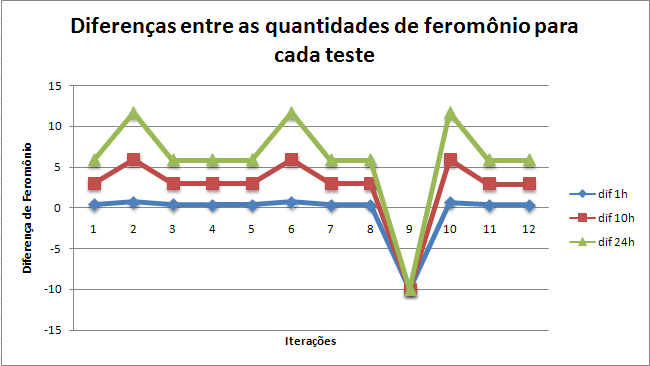
\includegraphics[width=10cm]{images/resultados/graf_diferencas.jpg}
                \label{fig:grafico:dif}
                \caption{Gr�fico indicativo com diferen�a de ferom�nio}
            \end{center}
        \end{figure}

\end{frame}
